\documentclass[a4paper,10pt]{article}
\usepackage[utf8x]{inputenc}

\usepackage{graphics}
\usepackage{amsmath}    % need for subequations
\usepackage{graphicx}   % need for figures
\usepackage{verbatim}   % useful for program listings
\usepackage{color}      % use if color is used in text
\usepackage{subfigure}  % use for side-by-side figures
\usepackage{hyperref}   % use for hypertext links, including those to external


%% Encabezado y Pie de Pagina %%

\makeindex

%opening
\title{Computaci\'on Gr\'afica \\Ray Tracer \\Grupo 2}
\author{Guillermo Campelo\\Juan Ignacio Go\~ni\\Juan Tenaillon\\Santiago
V\'azquez}

\begin{document}


\maketitle

\begin{abstract}
Dise\~namos y desarrollamos un motor de Ray Tracing, determinando
intersecciones entre rayos y objetos, considerando luminosidad, reflexiones,
refracciones, sombras, texturas y anti-aliasing. 
\end{abstract}

\section{Introducci\'on}
\label{intro}
A lo largo de este informe, detallaremos el dise\~no y desarrollo del motor de
Ray Tracing y explicaremos en detalle c\'omo decidimos implementar las distintas
partes que componen a la aplicaci\'on.

Para realizar el mismo, partimos del trabajo pr\'actico anterior, que
consisti\'o en
el desarrollo de un Ray Caster.  A partir del motor de ray casting,
construimos encima
el motor de ray tracing, que toma en consideraci\'on muchas cosas que el ray
caster no ten\'ia.
Entre estas cosas se encuentran las luces, sombras, reflecciones y refracciones,
texturas y la
posibilidad de tener movilidad en la c\'amara entre otras.

Adem\'as de explicar los detalles del dise\~no y de la implementaci\'on,
mostraremos imagenes generadas utilizando el motor haciendo uso de las distintas
opciones que presenta.

Tambi\'en desarrollamos t\'ecnicas de optimizaci\'on para hacer m\'as eficiente
al motor y, como resultado, generar im\'agenes de igual calidad a mayor
velocidad.  En nuestro caso, implementamos Octrees, debido a que nos brinda
tanto vol\'umenes envolventes como tambi\'en subdivisi\'on espacial.  Una
explicaci\'on m\'as detallada de esto podr\'a ser encontrada en la secci\'on
\ref{octree}.

En la secci\'on \ref{escena} detallaremos cada uno de los elementos que componen
a una escena, como las c\'amaras, las luces y los objetos que la pueblan.  En la
siguiente secci\'on, la \ref{motor}, explicaremos m\'as en detalle el motor de
ray tracing, explicando qu\'e es, c\'omo funciona, las caracter\'isticas del
mismo, las optimizaciones que decidimos implementar y una serie de pruebas
realizadas con el motor.
Por \'ultimo, en la secci\'on \ref{conc},
daremos nuestras conclusiones al respecto sobre el motor que implementamos.

\section{Escena}
\label{escena}
En esta secci\'on comentaremos las distintas partes que componen a la escena. 
Estas son las c\'amaras, las luces y los objetos mismos que la componen, como
los cubos, esferas y figuras complejas.

\subsection{C\'amara}

Desarrollamos dos tipos de c\'amaras distintas, $pinhole$ y $thinlens$.

La c\'amara $pinhole$ es la c\'amara est\'andar mientras que la c\'amara de
tipo $thinlens$ es la utilizada para modelar la profundidad del campo.

A los efectos de nuestro trabajo y el alcance del mismo, el tipo de c\'amara no
influye.

Una caracter\'istica intr\'inseca en la definici\'on de la c\'amara
utilizando $Sunflow$ es que es posible tener una c\'amara movil.  Esto nos
permite ver la misma escena desde difrentes perspectivas.  Esto lo apreciamos
en la figura \ref{fig:figure1} y \ref{fig:figure2}.

\begin{figure}[ht]
\begin{minipage}[b]{0.5\linewidth}
\centering
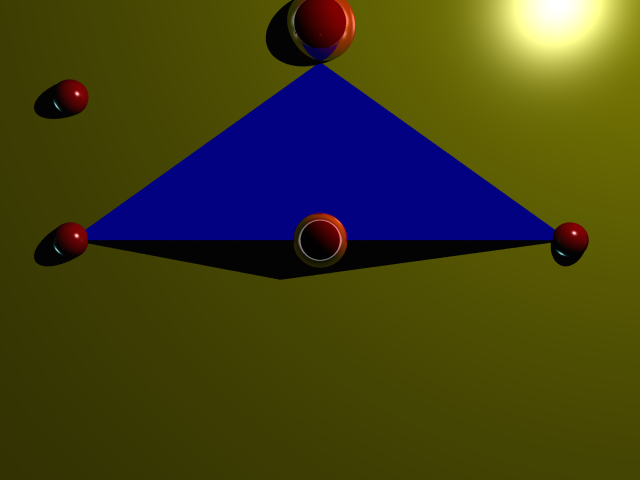
\includegraphics[scale=0.25]{scene1_a.png}
\caption{C\'amara en (0, 0, 20)}
\label{fig:figure1}
\end{minipage}
\hspace{0.5cm}
\begin{minipage}[b]{0.5\linewidth}
\centering
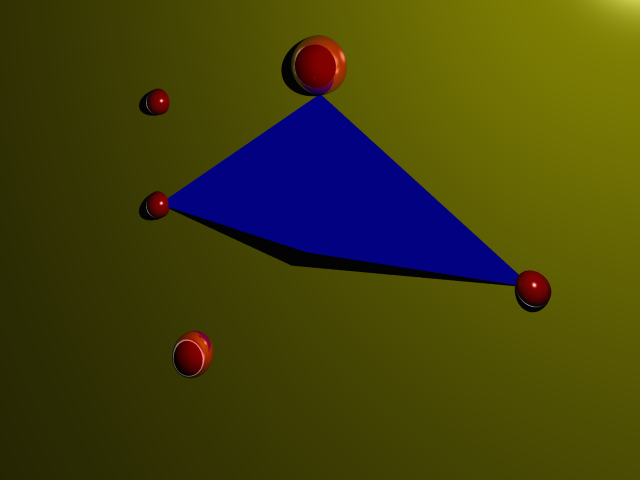
\includegraphics[scale=0.25]{scene1.png}
\caption{C\'amara en (10, 10, 20)}
\label{fig:figure2}
\end{minipage}
\end{figure}

\subsection{Luces}
\label{luces}
Las luces que implementamos fueron dos, una luz de ambiente y una luz puntual.

En caso de no haber una luz puntual definida, la luz ambiente entra en juego
para que se pueda apreciar algo de la escena.  Esto surgi\'o como una necesidad
ante la falta de luces puntuales en algunas escenas.  Decidimos implementar una
tenue luz ambiental para poder observar las escenas.

La implementaci\'on es simple.  Al no haber ninguna luz puntual definida en la
escena, el motor busca el color que deber\'ia tener el pixel y devuelve ese
valor oscurecido.

El otro tipo de luz implementada, es una luz puntual.  Esta nos permite obtener
escenas con sombras, refracciones y reflecciones en la imagen resultante.  La
luz cuenta con una posici\'on y una potencia y a medida que nos alejamos de
ella, la potencia disminuye.  Esta disminuci\'on fue inicialmente implementada
usando la ecuaci\'on \ref{eqn:luz}.

\begin{equation}
\label{eqn:luz}
Potencia de Luz (d_{punto-luz}) = \frac{P_{luz}}{ln( d_{punto-luz} + 1 ) + 1}
\end{equation}

Luego se decidi\'o usar una disminuci\'on lineal de la luz, ya que la f\'ormula
\ref{eqn:luz} nos daba una luz muy fuerte a\'un con una muy poca potencia. \'Esta ecuaci\'on
se puede ver en \ref{eqn:luzlineal}.

\begin{equation}
\label{eqn:luzlineal}
Potencia de Luz (d_{punto-luz}) = 1 - \frac{d_{punto-luz}}{P_{luz}}
\end{equation}


Obviamente, al existir una luz puntual, tambi\'en existen sombras.  Un pixel se
encuentra sombreado si hay alg\'un objeto opaco entre el punto y el centro de
la luz.  Si el objeto entre medio es transl\'ucido, el punto no estar\'a
sombreado.

Con este \'ultimo punto se nos present\'o un error que no fue f\'acil advertir.
 En caso de existir un objeto que intersecte el rayo entre el punto y la luz,
pero que no est\'e entre la luz y el punto, sino detr\'as de la luz, este pixel
aparec\'ia sombreado.  Luego de que advertimos cual era el problema, tuvimos
que realizar un c\'alculo extra para determinar si la distancia entre la
intersecci\'on con el objeto era mayor o menor que la distancia entre el punto
y la luz.

\begin{figure}[ht]
\begin{minipage}[b]{0.5\linewidth}
\centering

\includegraphics[scale=0.25]{scene5a.png}
\caption{Sin luz.}
\label{fig:figure3}
\end{minipage}
\hspace{0.5cm}
\begin{minipage}[b]{0.5\linewidth}
\centering
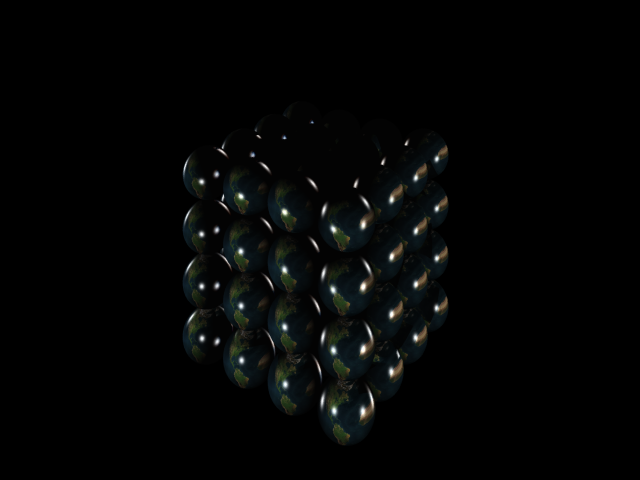
\includegraphics[scale=0.25]{scene5.png}
\caption{Con 3 luces.}
\label{fig:figure4}
\end{minipage}
\end{figure}

En la figura \ref{fig:figure3} observamos que se ve muy poco de los 64
mundos, mientras que en la figura \ref{fig:figure4} las observamos m\'as
claramente.

\subsection{Primitivas}

Las primitivas que desarrollamos fueron tres, estas son esferas, cubos,
tri\'angulos y planos.  De esta forma se pueden definir figuras m\'as
complejas, como explicamos a continuaci\'on, que son los $mesh$ o mallas de
tri\'angulos.

\subsubsection{Esferas}

El \'unico cambio con respecto a las esferas del primer trabajo pr\'actico, es
el hecho de que ac\'a utilizamos un eje imaginario para poder rotar la esfera.

Al crear una esfera, se calcula un eje para luego al rotarla poder calcular
qu\'e punto de la textura le pertenece.

Para leer una explicaci\'on de la intersecci\'on entre un rayo y la esfera,
leer el informe del Trabajo Pr\'actico \#1.

\subsubsection{Tri\'angulo}
La representaci\'on del triangulo y la intersecci\'on de un rayo con el mismo
lo comentamos en el informe del Trabajo Pr\'actico \#1.  Cuando desarrollamos
el motor de ray tracing, tuvimos que agregarle algunas cosas m\'as, como las
normales en cada punto y el mapeo con los puntos $UV$ para el caso del mapeo
con las texturas.

Para mapear las texturas en los tri\'angulos, con los 3 puntos que definen al
tri\'angulo, se crean 2 vectores, entre uno de los puntos y los otros dos, que
forman una base para el plano sobre el cual est\'a el tri\'angulo.
Con estos vectores, su punto inicial y el punto contra el que hizo
intersecci\'on el rayo emitido, se toma el componente que multiplica a cada uno
de los vectores de la base, que var\'ia entre $0$ y $1$ obteniendo as\'i, los
valores de u y v contra los que se mapea en la textura el punto de
intersecci\'on.

Por otro lado, las transformaciones en los tri\'angulos son simples.  Al
momento de aplicarle una traslaci\'on, una rotaci\'on o un escalamiento, se
multiplican los tres puntos del tri\'angulo por una matriz determinada por la
acci\'on a tomar, y luego se recalculan las dem\'as variables como las normales
y los puntos de mapeo.

\subsubsection{Cubos}

Para implementar el cubo decidimos usar doce tri\'angulos.  De esta forma, el
problema de la intersecci\'on queda resuelto.  Por otro lado, para realizar las
transformaciones de la primitiva, se utiliza el mismo concepto, se transforman
los doce tri\'angulo uno a uno.

Por definici\'on, un cubo es de lado 1 y est\'a en el origen de coordenadas, y
mediante las transformaciones, podemos moverlo hacia otro punto de la escena, 
rotarlo y escalarlo.

En el caso de las texturas, considerando que los cubos en s\'i, est\'an
formados por 12 tri\'angulos, 2 por cada cara del mismo. Al ser en s\'i
tri\'angulos, la textura ya esta resuelta. El \'unico obst\'aculo a superar fue
la correcta ubicaci\'on de los tri\'angulos para que conicidan las texturas.

\subsubsection{Planos}

Tambi\'en implementamos planos.  Para hacerlo, lo definimos como un punto y una
normal.  De esta forma, el c\'alculo de la intersecci\'on de un rayo con el
mismo se simplifica.  El c\'alculo utilizado es el mismo que para los
tri\'angulos, pero sin determinar si el punto pertenece al al mismo.

Tambi\'en es posible mapear texturas al plano.  De igual forma que con los
tri\'angulos se crean 2 vectores utilizando el punto con el que se construye el
plano y la normal del mismo. Con dichos vectores se toman los componentes u y v
para el mapeo contra la textura.

Pero surge un inconveniente, el plano tiene largo infinito, por lo que no se
puede tomar ninguna referencia como un punto m\'aximo o m\'inimo para
corresponder con el m\'aximo y m\'inimo de la textura. La soluci\'on que
encontramos para esto, fue hacer una repetici\'on de la textura por cada cierto
tama\~no fijo.


\subsubsection{Figuras Complejas}

Para realizar figuras complejas, utilizamos las mallas de tri\'angulos. 
Mediante la creaci\'on de muchos tri\'angulos, es posible generar objetos que
no pueden formarse como primitivas en s\'i.  Un ejemplo claro de esto, es el el
alambre o la torre de agua que podemos ver en las figuras \ref{fig:figure5} y
\ref{fig:figure6}.

\begin{figure}[ht]
\begin{minipage}[b]{0.5\linewidth}
\centering
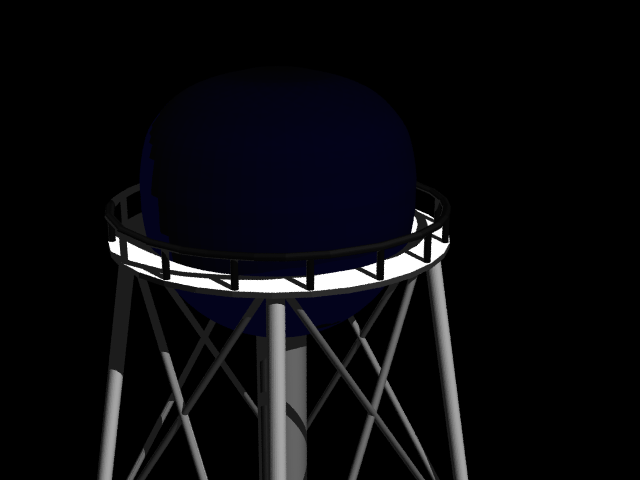
\includegraphics[scale=0.25]{watertower.png}
\caption{Torre de Agua.}
\label{fig:figure5}
\end{minipage}
\hspace{0.5cm}
\begin{minipage}[b]{0.5\linewidth}
\centering
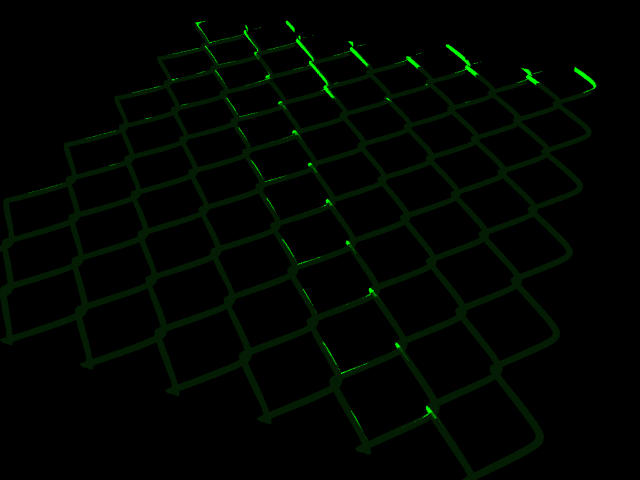
\includegraphics[scale=0.25]{chainlink.png}
\caption{Alambre.}
\label{fig:figure6}
\end{minipage}
\end{figure}

En el caso de los mapeos de las texturas, este punto queda resuelto al igual
que en los tri\'angulos, ya que estas figuras complejas son conjuntos de
tri\'angulos.


\section{Motor de Ray Tracing}
\label{motor}

\subsection{Anti Aliasing}
El \emph{anti aliasing} fue resuelto con la creaci\'on de varios rayos por cada
pixel en la imagen. Dos par\'ametros determinan la cantidad y disposici\'on de
los rayos. Se toma el mayor n\'umero del par\'ametro \emph{aa} para saber la
potencia de $2$ subdivisiones horizontales y verticales para cada pixel, es
decir, si el n\'umero es $2$, se deben crear $2$ por $2$ zonas dentro del pixel
en las que se deben tirar tantos rayos como el par\'ametro \emph{samples}
determine.

Los rayos creados se lanzan en forma estoc\'astica dentro de los l\'imites
creados por las subdivisiones para darle un nivel de realismo a la imagen
generada.

En la figura \ref{fig:figure7} observamos la diferencia entre usar
\emph{anti alisasing} y no usarlo.  Adem\'as, en el figura \ref{fig:figure8}
observamos c\'omo se subdivide el espacio y por cada divisi\'on disparamos
m\'as rayos que en caso de no utilizar \emph{anti aliasing}.

\begin{figure}[ht]
\begin{minipage}[b]{0.5\linewidth}
\centering
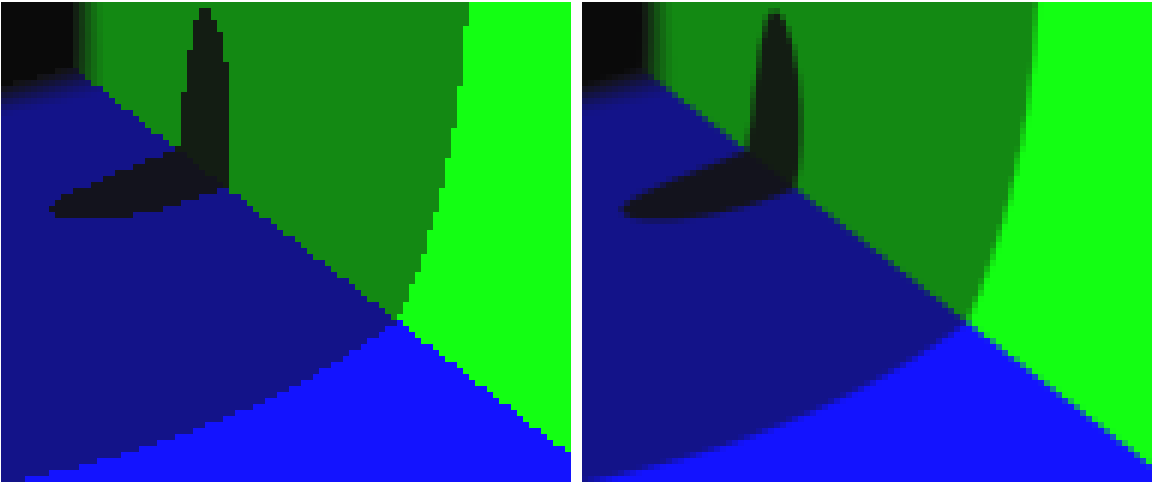
\includegraphics[scale=0.23]{aa_muestra.png}
\caption{Ejemplo de Anti Aliasing}
\label{fig:figure7}
\end{minipage}
\hspace{0.5cm}
\begin{minipage}[b]{0.5\linewidth}
\centering
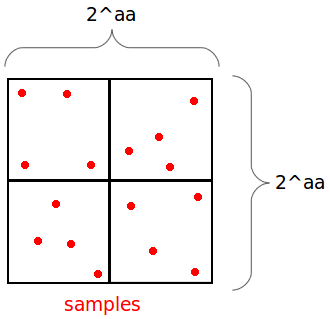
\includegraphics[scale=0.40]{aa_samples.png}
\caption{Divisi\'on del Pixel}
\label{fig:figure8}
\end{minipage}
\end{figure}

\subsection{Sombras}

C\'omo explicamos en la secci\'on \ref{luces}, las sombras se determinan si
existen objetos entre la luz y el punto.  En caso de haber un objeto bloqueando
la luz, ese pixel quedar\'a sombreado, en cambio, si no hay objetos entre la
luz y el punto, el pixel no estar\'a sombreado.

Decidimos implementar \emph{soft shadows}, que suaviza un poco las sombras en
los puntos cercanos a los expuestos a la luz. Para \'esto se crearon luces adicionales
alrededor de cada luz de la escena, de forma tal que se generen varias sombras a
partir de una luz y as\'i dar un efecto de una sombra m\'as suave. Claramente, 
esto aumenta el tiempo de rendering, ya que aumenta la cantidad de luces en
la escena.

En las figuras \ref{fig:figure9} y \ref{fig:figure10} observamos un ejemplo
de sombras suaves y sombras simples respectivamente.

\begin{figure}[ht]
\begin{minipage}[b]{0.5\linewidth}
\centering
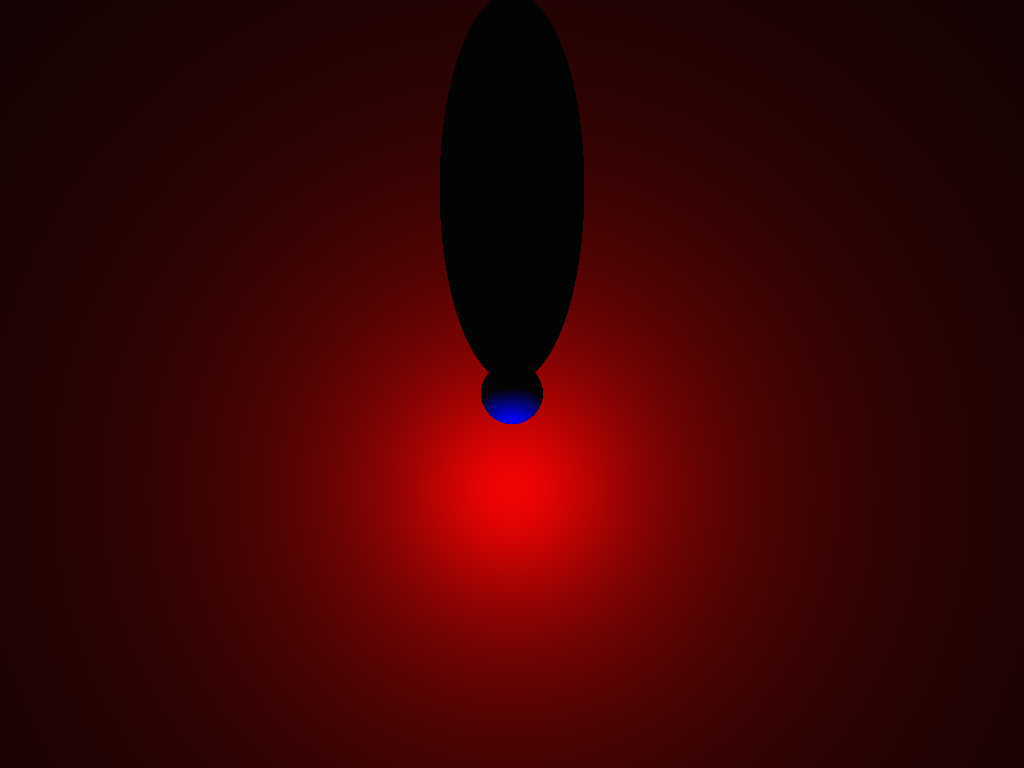
\includegraphics[scale=0.17]{scene21.png}
\caption{Sombras suaves.}
\label{fig:figure9}
\end{minipage}
\hspace{0.5cm}
\begin{minipage}[b]{0.5\linewidth}
\centering
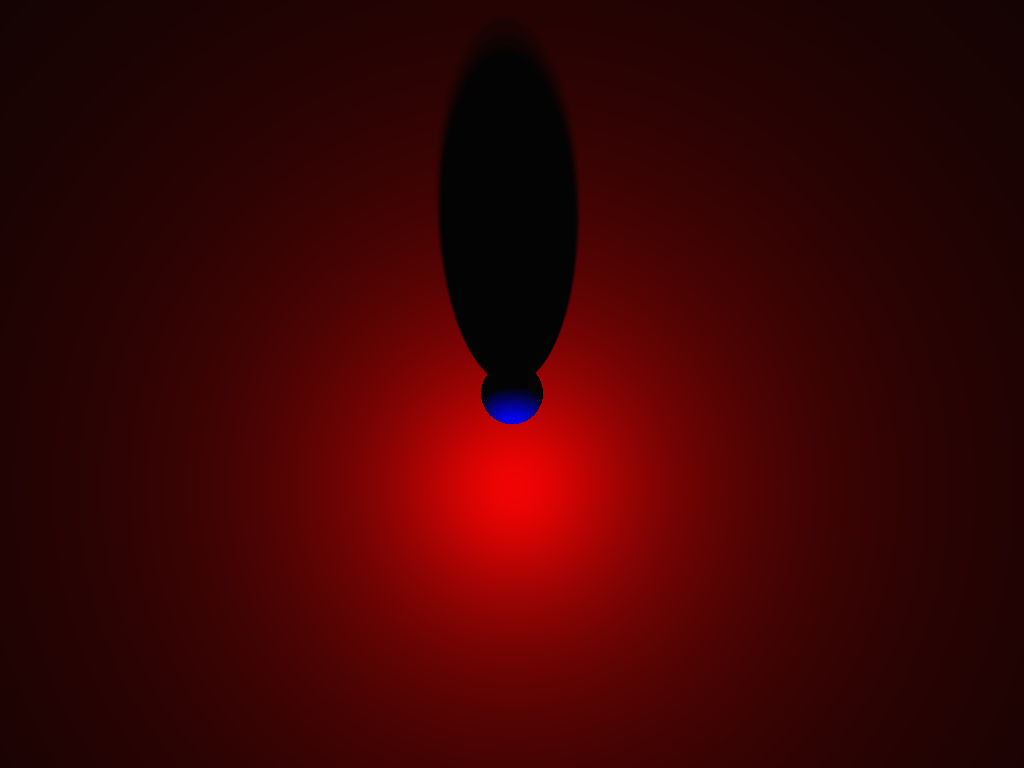
\includegraphics[scale=0.17]{scene21soft.png}
\caption{Sombras simples.}
\label{fig:figure10}
\end{minipage}
\end{figure}

\subsection{Shaders}

Implementamos cuatro shaders distintos, \emph{constant}, \emph{phong},
\emph{glass} y \emph{mirror}.  Decidimos implementar uno m\'as que los
requeridos para poder probar las escenas de prueba de la c\'atedra, ya que
muchas de ellas no contaban con un shader de los pedidos definido.  A
continuaci\'on explicamos cada uno de ellos.

\subsubsection{Constant}
Se implement\'o el shader \emph{constant} para poder representar las escenas de
prueba entregadas por la c\'atedra. Este shader simple consta de un color que
esta distribuido de forma uniforme en la superficie de la primitiva.

\subsubsection{Phong}
En el caso de querer utilizar una textura sobre una figura, hay que utilizar
\emph{phong}, aunque tambi\'en se le puede especificar un color difuso en 
vez de una textura por si se requiere. Este shader cuenta con una imagen
que luego es utilizada para mapear a los distintos objetos.
Tambi\'en cuenta con un coeficiente de especularidad, que determina cu\'anto
influye el valor especular de la superficie en el color de reflejo de la misma.

En la figura \ref{fig:figure11} se puede observar una esfera con una textura,
la tierra en este caso.  Adem\'as, podemos observar como tiene un cierto
reflejo, dado por el coeficiente de especularidad asignado en este caso.

\begin{figure}[ht]
\centering
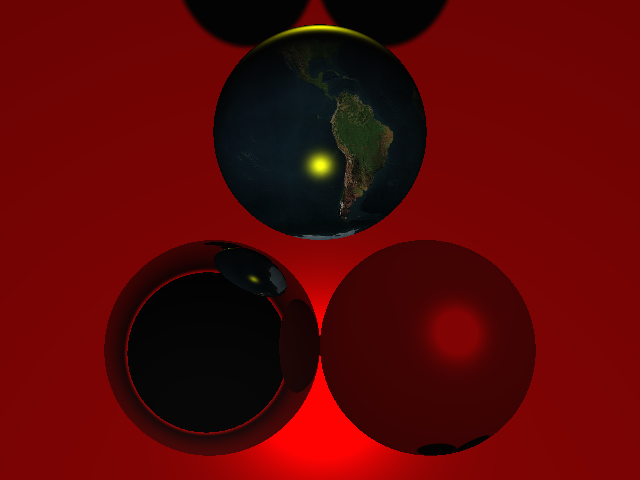
\includegraphics[scale=0.50]{earth.png}
\caption{Esferas texturadas utilizando \emph{phong}.}
\label{fig:figure11}
\end{figure}

\subsubsection{Glass}

Este tipo de shader lo utilizamos cuando queremos que la figura en cuesti\'on
sea traslucida.  Para este tipo de shader hay que definir un \'indice de
refracci\'on que ser\'a utilizado para calcular la direcci\'on en la que sale el
nuevo rayo una vez que intersecta.

En la figura \ref{fig:figure12} se puede observar una serie de figuras con unos
planos de fondo.  Observamos claramente que las esferas son traslucidas y se
puede ver detr\'as de ellas.

\begin{figure}[ht]
\centering
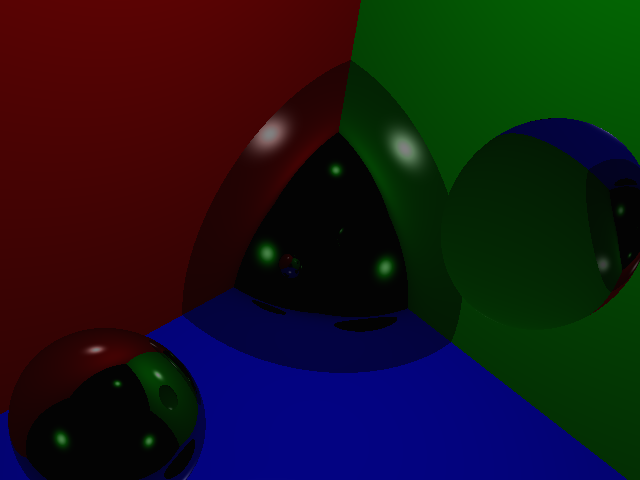
\includegraphics[scale=0.50]{scene4.png}
\caption{Esferas utilizando \emph{glass}, \emph{mirror} y planos.}
\label{fig:figure12}
\end{figure}

\subsubsection{Mirror}

Este tipo de shader lo utilizamos cuando queremos que el objeto refleje como un
espejo.  En este caso debemos definir un coeficiente de reflexi\'on ya que los
rayos, al golpear ser\'an reflejados en lugar de atravesar la figura.

En la figura \ref{fig:figure12} podemos observar una esfera que utiliza como
shader un mirror.

\section{Optimizaciones y Opcionales}
Decidimos implementar algunas optimizaciones al algoritmo para hacerlo m\'as
eficiente.  Tuvimos que implementar un sistema de subdivisi\'on espacial y de
vol\'umenes envolventes y fue por eso que elegimos \emph{octree}.
\subsection{Subdivisi\'on Espacial y Vol\'umenes Envolventes}
\label{octree}


\subsection{Multi Threading}

Implementamos tambi\'en multiples hilos de ejecuci\'on.  Esto optimiza el poder
de los procesadores de varios n\'ucleos de hoy en d\'ia y agiliza al motor de
ray tracing.

En la secci\'on \ref{bench} podemos observar las mejoras respecto a la
ejecuci\'on con solo un hilo.

\subsection{Progress Bar}

Se implement\'o para informar el progreso del render, un informe progresivo de
la cantidad de trabajos o \emph{buckets} realizados en forma de porcentaje
completado. Esto ayuda en gran medida a la hora de realizar renders de escenas
complejas en cantidad de primitivas o efectos sobre las mismas.

\section{Benchmarking}
\label{bench}
\section{Conclusiones}
\label{conc}

Del desarrollo del motor concluimos que, de manera relativamente simple, es
posible realizar renders de im\'agenes de muy alta calidad en tiempos
razonables.  Los tiempos razonables son debido a las optimizaciones
implementadas, dado que sin ellas los tiempos eran muy mayores.

Tambi\'en se demuestra a las claras que las t\'ecnicas de anti aliasing y
sombras suaves ayudar a mejorar a\'un m\'as la imagen, que se present\'a con
menos brusquedad en los cambios de color entre una figura y la otra.  El
refinamiento de los pixeles de la imagen retarda un poco m\'as el render, pero
el resultado es bastante mejor que no usarlo.

Por supuesto, hay que considerar que todas estas cuestiones se engloban bajo la
disyuntiva entre el tiempo insumido y la calidad que queremos obtener.  A m\'as
calidad, m\'as tiempo ser\'a necesario y lo inverso tambi\'en se cumple.





\end{document}
